\documentclass[a4paper,14pt]{report}
\usepackage[utf8]{inputenc}
\usepackage[T1]{fontenc}
\usepackage{amsmath}
\usepackage{float}
\usepackage{graphicx}
\graphicspath{ {./wykresy/} }
\title{Wprowadzenie do sztucznej inteligencji, Lista 3}
\author{Radosław Wojtczak}
\date{254607}
\begin{document}
\maketitle
\section{Wprowadzenie}
	Celem zadania było wykorzystanie zbioru danych \textbf{THE MNIST DATABASE of handwritten digits} do wykonania klasteryzacji metodą k-średnich. Do wykonania tego zadania skorzystałem z biblioteki \textit{sklearn}, z metody \textit{KMeans}
\section{Rozwiązanie}
	Ów program został napisany w języku programowania python, przy pomocy narzędzia "Google Colab".
	Dokonujemy wszystkie potrzebne importy włącznie z danymi z MNIST DATABASE, które dostępne są w pakiecie \textit{tensorflow}. Następnie dokonujemy konwersji danych i w pętli od $k=7$ do $k=13$ wykonujemy funkcję \textit{KMeans} w celu wytrenowania zbioru. W każdym obrocie pętli wykonujemy funkcję \textit{Kmeans} z innym parametrem inicjucjącym, \textit{k-means++} lub \textit{random}, po czym algorytm pracuje dalej z wersją, której inercja jest \textbf{mniejsza}. \\
	Dodatkowo dokonano dwóch typów testów:
	\begin{itemize}
		\item W pierwszym teście zamieniono zbiór testowy z treningowym ze względu na czas trenowania (10000 elementów treningowych, 60000 testowych)
		\item W drugim teście wykonano trening na zbiorze pierwotnym (60000 elementów treningowych, 10000 testowych)
	\end{itemize}
	Poniżej znajduja się wyniki otrzymane w ramach rozwiązania zadania. Ostatecznie zdecydowałem się rozszerzyć wymagania i każdy z podpunktów przetestować dla wszystkich podanych w treści wartości $k$.
	Zaprezentowane wyniki są przykładowym wywołaniem, ze względu na liczność testów postanowiłem szczegółowo przedstawić wyniki jedynie jednego z przykładowych.

\section{Otrzymane wyniki dla mniejszego zbioru}
	\textbf{Dane dla k=7: } \\
	Porównanie inercji: 
	\begin{itemize}
		\item K-means: 410910.5
		\item Random: 410911.625
	\end{itemize}
	Wybrana metoda- "K-means" \\
	Przedstawienie graficzne jako macierz 7 na 10 rozkładu procentowego przydziału cyfr do poszczególnych klastrów:
	(UWAGA: Ze względu na zastosowane zaokrąglenie (2 liczby po przecinku) suma wiersza nie zawsze musi równać się $100\%$ (lecz jest do tej wartości zbliżona))
	\begin{itemize}
		\item Test:
		$
		\begin{bmatrix}
		2.28\% & 2.58\% & 72.1\% & 8.14\% & 0.3\% & 1.69\% & 1.99\% & 1.89\% & 8.84\% & 0.2\% \\
		3.64\% & 0.31\% & 3.38\% & 41.64\% & 0.0\% & 23.9\% & 1.23\% & 0.0\% & 25.08\% & 0.82\% \\
		0.23\% & 62.64\% & 8.71\% & 3.47\% & 2.16\% & 6.55\% & 4.33\% & 4.61\% & 5.93\% & 1.37\% \\
		2.9\% & 0.32\% & 3.1\% & 0.75\% & 3.43\% & 1.61\% & 86.0\% & 0.0\% & 1.29\% & 0.64\% \\
		91.07\% & 0.0\% & 2.18\% & 0.44\% & 0.44\% & 0.98\% & 2.61\% & 0.11\% & 1.09\% & 1.09\% \\
		0.85\% & 0.0\% & 0.74\% & 1.48\% & 18.4\% & 11.56\% & 0.11\% & 32.45\% & 12.67\% & 21.74\% \\
		0.19\% & 0.0\% & 1.55\% & 1.03\% & 36.02\% & 3.36\% & 0.58\% & 20.34\% & 2.0\% & 34.93\% \\
		\end{bmatrix} 
		$
		\item Train:
		$
		\begin{bmatrix}
		2.98\% & 2.05\% & 69.57\% & 8.95\% & 0.54\% & 1.34\% & 2.69\% & 0.91\% & 10.81\% & 0.16\% \\
		3.26\% & 0.19\% & 3.23\% & 42.7\% & 0.02\% & 25.07\% & 1.3\% & 0.04\% & 23.14\% & 1.05\% \\
		0.31\% & 58.17\% & 7.08\% & 4.07\% & 2.5\% & 7.84\% & 6.21\% & 4.04\% & 7.81\% & 1.96\% \\
		3.12\% & 0.11\% & 3.53\% & 0.86\% & 3.6\% & 1.62\% & 85.84\% & 0.11\% & 0.9\% & 0.31\% \\
		91.73\% & 0.0\% & 1.66\% & 0.73\% & 0.26\% & 1.5\% & 1.74\% & 0.5\% & 0.8\% & 1.1\% \\
		1.15\% & 0.13\% & 0.9\% & 1.62\% & 18.47\% & 10.32\% & 0.09\% & 32.12\% & 12.75\% & 22.46\% \\
		0.21\% & 0.12\% & 1.64\% & 2.16\% & 35.13\% & 3.83\% & 0.45\% & 21.87\% & 2.26\% & 32.33\% \\
		\end{bmatrix} 
		$
	\end{itemize}
	Otrzymane wyniki procentowe:
	\begin{itemize}
		\item Zbiór treningowy z bazy danych MNIST: $3.85\%$ ($\frac{2311}{60000}$)
		\item Zbiór własnoręczny: $10.0\%$ ($\frac{5}{50}$)
	\end{itemize}
	\textbf{Dane dla k=8: } \\
	Porównanie inercji: 
	\begin{itemize}
		\item K-means: 402989.5625
		\item Random: 402998.5
	\end{itemize}
	Wybrana metoda- "Random" \\
	Przedstawienie graficzne jako macierz 8 na 10 rozkładu procentowego przydziału cyfr do poszczególnych klastrów:
	(UWAGA: Ze względu na zastosowane zaokrąglenie (2 liczby po przecinku) suma wiersza nie zawsze musi równać się $100\%$ (lecz jest do tej wartości zbliżona))
	\begin{itemize}
		\item Test:
		$
		\begin{bmatrix}
		0.13\% & 0.0\% & 0.93\% & 0.73\% & 22.63\% & 4.51\% & 0.13\% & 41.87\% & 3.12\% & 25.95\% \\
		0.35\% & 64.01\% & 7.56\% & 3.49\% & 2.38\% & 7.15\% & 3.84\% & 4.53\% & 5.0\% & 1.69\% \\
		4.03\% & 0.22\% & 5.80\% & 52.94\% & 0.0\% & 20.93\% & 0.15\% & 0.0\% & 15.35\% & 0.59\% \\
		0.19\% & 0.0\% & 1.43\% & 1.17\% & 35.93\% & 3.57\% & 0.52\% & 19.39\% & 2.33\% & 35.47\% \\
		2.51\% & 0.33\% & 2.61\% & 0.64\% & 3.92\% & 1.42\% & 87.03\% & 0.0\% & 0.87\% & 0.65\% \\
		92.53\% & 0.0\% & 1.93\% & 0.45\% & 0.23\% & 0.68\% & 2.38\% & 0.11\% & 0.79\% & 0.91\% \\
		5.6\% & 0.41\% & 1.34\% & 11.95\% & 0.25\% & 27.99\% & 3.59\% & 0.08\% & 47.37\% & 1.42\% \\
		0.8\% & 2.64\% & 83.81\% & 5.4\% & 0.57\% & 0.8\% & 1.95\% & 2.07\% & 1.61\% & 0.34\% \\
		\end{bmatrix} 
		$
		\item Train:
		$
		\begin{bmatrix}
		0.33\% & 0.12\% & 0.98\% & 0.63\% & 22.53\% & 3.48\% & 0.03\% & 41.94\% & 2.65\% & 27.31\% \\
		0.31\% & 59.82\% & 6.28\% & 3.86\% & 2.81\% & 8.37\% & 5.88\% & 4.1\% & 6.27\% & 2.3\% \\
		2.89\% & 0.17\% & 5.25\% & 52.7\% & 0.0\% & 21.96\% & 0.60\% & 0.65\% & 15.3\% & 1.05\% \\
		0.2\% & 0.16\% & 1.57\% & 2.28\% & 35.32\% & 4.11\% & 0.41\% & 20.44\% & 2.58\% & 32.92\% \\
		2.85\% & 0.11\% & 3.21\% & 0.74\% & 4.03\% & 1.51\% & 86.29\% & 0.11\% & 0.84\% & 0.29\% \\
		92.49\% & 0.0\% & 1.65\% & 0.55\% & 0.28\% & 1.27\% & 1.59\% & 0.47\% & 0.64\% & 1.06\% \\
		6.93\% & 0.20\% & 1.64\% & 14.01\% & 0.49\% & 26.6\% & 3.44\% & 0.08\% & 45.54\% & 1.07\% \\
		1.35\% & 1.87\% & 83.71\% & 6.14\% & 0.79\% & 0.57\% & 2.38\% & 1.12\% & 1.85\% & 0.2\% \\
		\end{bmatrix} 
		$
	\end{itemize}
	Otrzymane wyniki procentowe:
	\begin{itemize}
		\item Zbiór treningowy z bazy danych MNIST: $13.03\%$ ($\frac{7819}{60000}$)
		\item Zbiór własnoręczny: $10.0\%$ ($\frac{5}{50}$)
	\end{itemize}
	\textbf{Dane dla k=9: } \\
	Porównanie inercji: 
	\begin{itemize}
		\item K-means: 395662.1875
		\item Random: 395662.21875
	\end{itemize}
	Wybrana metoda- "K-means" \\
	Przedstawienie graficzne jako macierz 9 na 10 rozkładu procentowego przydziału cyfr do poszczególnych klastrów:
	(UWAGA: Ze względu na zastosowane zaokrąglenie (2 liczby po przecinku) suma wiersza nie zawsze musi równać się $100\%$ (lecz jest do tej wartości zbliżona))
	\begin{itemize}
		\item Test:
		$
		\begin{bmatrix}
		1.23\% & 0.0\% & 84.83\% & 5.67\% & 0.86\% & 0.86\% & 2.96\% & 1.73\% & 1.48\% & 0.37\% \\
		0.2\% & 0.0\% & 1.0\% & 0.73\% & 22.1\% & 6.04\% & 0.13\% & 40.94\% & 3.05\% & 25.81\% \\ 
		4.07\% & 0.22\% & 5.99\% & 52.81\% & 0.0\% & 21.08\% & 0.15\% & 0.07\% & 15.09\% & 0.52\% \\ 
		0.58\% & 56.45\% & 13.24\% & 0.93\% & 3.25\% & 9.52\% & 1.86\% & 6.5\% & 6.39\% & 1.28\% \\
		92.84\% & 0.0\% & 1.82\% & 0.45\% & 0.11\% & 0.57\% & 2.5\% & 0.11\% & 0.8\% & 0.8\% \\ 
		0.0\% & 67.47\% & 5.46\% & 6.61\% & 3.25\% & 2.52\% & 4.83\% & 4.41\% & 2.94\% & 2.52\% \\ 
		5.3\% & 0.08\% & 1.66\% & 11.75\% & 0.17\% & 27.81\% & 3.97\% & 0.08\% & 47.85\% & 1.32\% \\ 
		0.2\% & 0.0\% & 1.63\% & 1.05\% & 35.92\% & 3.27\% & 0.65\% & 19.33\% & 2.35\% & 35.6\% \\ 
		2.56\% & 0.22\% & 2.34\% & 0.67\% & 3.34\% & 1.34\% & 87.85\% & 0.0\% & 0.89\% & 0.78\% \\ 
		\end{bmatrix} 
		$
		\item Train:
		$
		\begin{bmatrix}
		1.82\% & 0.17\% & 85.41\% & 5.81\% & 0.81\% & 0.64\% & 2.77\% & 0.93\% & 1.38\% & 0.27\% \\ 
		0.35\% & 0.11\% & 0.95\% & 0.68\% & 21.98\% & 4.8\% & 0.03\% & 41.39\% & 2.64\% & 27.07\% \\ 
		2.95\% & 0.17\% & 5.18\% & 52.79\% & 0.0\% & 22.04\% & 0.65\% & 0.07\% & 15.12\% & 1.03\% \\ 
		0.35\% & 54.28\% & 8.79\% & 1.84\% & 4.79\% & 11.2\% & 3.4\% & 5.16\% & 8.26\% & 1.93\% \\ 
		92.71\% & 0.0\% & 1.46\% & 0.53\% & 0.27\% & 1.29\% & 1.61\% & 0.47\% & 0.66\% & 1.0\% \\ 
		0.1\% & 62.39\% & 5.73\% & 6.58\% & 2.41\% & 3.25\% & 7.51\% & 4.34\% & 4.36\% & 3.34\% \\ 
		6.56\% & 0.11\% & 1.63\% & 14.17\% & 0.29\% & 26.47\% & 3.71\% & 0.05\% & 46.04\% & 0.98\% \\ 
		0.24\% & 0.07\% & 1.78\% & 2.19\% & 35.52\% & 4.04\% & 0.5\% & 20.35\% & 2.32\% & 32.99\% \\ 
		2.87\% & 0.07\% & 2.98\% & 0.74\% & 3.59\% & 1.48\% & 87.11\% & 0.09\% & 0.78\% & 0.28\% \\
		\end{bmatrix} 
		$
	\end{itemize}
	Otrzymane wyniki procentowe:
	\begin{itemize}
		\item Zbiór treningowy z bazy danych MNIST: $4.83\%$ ($\frac{2899}{60000}$)
		\item Zbiór własnoręczny: $14.0\%$ ($\frac{7}{50}$)
	\end{itemize}
	\textbf{Dane dla k=10: } \\
	Porównanie inercji: 
	\begin{itemize}
		\item K-means: 389395.6875
		\item Random: 389396.0625
	\end{itemize}
	Wybrana metoda- "K-means" \\
	Przedstawienie graficzne jako macierz 10 na 10 rozkładu procentowego przydziału cyfr do poszczególnych klastrów:
	(UWAGA: Ze względu na zastosowane zaokrąglenie (2 liczby po przecinku) suma wiersza nie zawsze musi równać się $100\%$ (lecz jest do tej wartości zbliżona))
	\begin{itemize}
		\item Test:
		$
		\begin{bmatrix}
		0.0\% & 67.22\% & 5.43\% & 6.78\% & 2.71\% & 3.86\% & 5.43\% & 3.24\% & 3.34\% & 1.98\% \\ 
		5.02\% & 0.08\% & 1.92\% & 14.88\% & 0.17\% & 26.17\% & 3.85\% & 0.08\% & 46.74\% & 1.09\% \\ 
		0.08\% & 0.0\% & 0.68\% & 0.59\% & 18.65\% & 2.03\% & 0.0\% & 40.08\% & 2.11\% & 35.78\% \\ 
		1.77\% & 0.0\% & 1.58\% & 1.02\% & 25.09\% & 13.85\% & 0.37\% & 31.32\% & 7.62\% & 17.38\% \\ 
		4.27\% & 0.23\% & 4.66\% & 52.68\% & 0.0\% & 22.07\% & 0.23\% & 0.0\% & 15.31\% & 0.54\% \\ 
		2.6\% & 0.23\% & 2.49\% & 0.68\% & 2.15\% & 1.36\% & 89.38\% & 0.0\% & 0.79\% & 0.34\% \\ 
		0.14\% & 65.9\% & 16.3\% & 0.27\% & 1.77\% & 2.99\% & 1.22\% & 6.11\% & 4.62\% & 0.68\% \\ 
		0.3\% & 0.0\% & 2.29\% & 1.09\% & 42.49\% & 3.88\% & 1.39\% & 12.64\% & 1.99\% & 33.93\% \\ 
		0.63\% & 0.0\% & 87.15\% & 6.05\% & 0.38\% & 0.76\% & 2.14\% & 1.26\% & 1.39\% & 0.25\% \\ 
		92.6\% & 0.0\% & 1.71\% & 0.46\% & 0.11\% & 0.68\% & 2.51\% & 0.23\% & 0.8\% & 0.91\% \\
		\end{bmatrix} 
		$
		\item Train:
		$
		\begin{bmatrix}
		0.1\% & 61.95\% & 6.05\% & 6.48\% & 2.22\% & 4.42\% & 8.27\% & 3.34\% & 4.82\% & 2.35\% \\ 
		6.36\% & 0.1\% & 1.71\% & 16.73\% & 0.15\% & 25.19\% & 3.63\% & 0.06\% & 45.37\% & 0.71\% \\ 
		0.11\% & 0.17\% & 0.69\% & 1.36\% & 19.4\% & 1.91\% & 0.02\% & 40.73\% & 1.74\% & 33.88\% \\ 
		1.98\% & 0.07\% & 1.88\% & 0.97\% & 23.22\% & 13.04\% & 0.47\% & 31.77\% & 6.93\% & 19.67\% \\ 
		3.19\% & 0.16\% & 4.51\% & 52.83\% & 0.0\% & 22.48\% & 0.6\% & 0.07\% & 15.03\% & 1.12\% \\ 
		2.83\% & 0.08\% & 2.86\% & 0.77\% & 2.37\% & 1.53\% & 88.64\% & 0.11\% & 0.66\% & 0.15\% \\ 
		0.11\% & 66.22\% & 10.29\% & 1.43\% & 2.3\% & 4.57\% & 2.67\% & 4.25\% & 7.22\% & 0.95\% \\ 
		0.35\% & 0.07\% & 2.44\% & 2.01\% & 41.1\% & 4.45\% & 1.17\% & 14.12\% & 2.41\% & 31.88\% \\ 
		1.1\% & 0.19\% & 87.41\% & 5.73\% & 0.42\% & 0.53\% & 2.38\% & 0.57\% & 1.44\% & 0.21\% \\ 
		93.2\% & 0.0\% & 1.5\% & 0.54\% & 0.21\% & 1.21\% & 1.59\% & 0.31\% & 0.58\% & 0.86\% \\
		\end{bmatrix} 
		$
	\end{itemize}
	Otrzymane wyniki procentowe:
	\begin{itemize}
		\item Zbiór treningowy z bazy danych MNIST: $2.17\%$ ($\frac{1301}{60000}$)
		\item Zbiór własnoręczny: $10.0\%$ ($\frac{5}{50}$)
	\end{itemize}
	\textbf{Dane dla k=11: } \\
	Porównanie inercji: 
	\begin{itemize}
		\item K-means: 383413.75
		\item Random: 383463.25
	\end{itemize}
	Wybrana metoda- "K-means" \\
	Przedstawienie graficzne jako macierz 11 na 10 rozkładu procentowego przydziału cyfr do poszczególnych klastrów:
	(UWAGA: Ze względu na zastosowane zaokrąglenie (2 liczby po przecinku) suma wiersza nie zawsze musi równać się $100\%$ (lecz jest do tej wartości zbliżona))
	\begin{itemize}
		\item Test:
		$
		\begin{bmatrix}
		0.83\% & 0.1\% & 3.62\% & 13.64\% & 0.0\% & 15.91\% & 0.21\% & 0.1\% & 64.46\% & 1.14\% \\ 
		0.0\% & 73.6\% & 5.6\% & 6.06\% & 2.29\% & 2.51\% & 1.94\% & 3.54\% & 2.4\% & 2.06\% \\
		0.36\% & 0.0\% & 3.31\% & 1.18\% & 44.26\% & 3.43\% & 2.01\% & 11.6\% & 1.54\% & 32.31\% \\ 
		0.26\% & 62.15\% & 14.71\% & 0.77\% & 2.69\% & 5.37\% & 1.02\% & 6.14\% & 6.01\% & 0.9\% \\
		1.7\% & 0.14\% & 1.98\% & 0.14\% & 2.41\% & 0.99\% & 91.78\% & 0.0\% & 0.71\% & 0.14\% \\ 
		93.32\% & 0.0\% & 1.54\% & 0.0\% & 0.13\% & 0.39\% & 2.7\% & 0.13\% & 0.9\% & 0.9\% \\ 
		20.28\% & 0.0\% & 2.8\% & 6.53\% & 2.45\% & 31.35\% & 27.16\% & 0.12\% & 8.51\% & 0.82\% \\ 
		0.26\% & 0.0\% & 91.96\% & 4.35\% & 0.0\% & 0.26\% & 0.66\% & 1.32\% & 0.92\% & 0.26\% \\ 
		0.17\% & 0.0\% & 0.75\% & 0.92\% & 21.67\% & 2.5\% & 0.17\% & 35.17\% & 1.33\% & 37.33\% \\ 
		4.27\% & 0.25\% & 3.1\% & 58.46\% & 0.0\% & 23.95\% & 0.34\% & 0.0\% & 9.05\% & 0.59\% \\ 
		0.0\% & 0.0\% & 1.06\% & 0.97\% & 25.89\% & 4.64\% & 0.1\% & 40.19\% & 5.12\% & 22.03\% \\
		\end{bmatrix} 
		$
		\item Train:
		$
		\begin{bmatrix}
		0.85\% & 0.19\% & 3.43\% & 15.43\% & 0.11\% & 15.84\% & 0.35\% & 0.13\% & 62.7\% & 0.96\% \\ 
		0.06\% & 69.5\% & 6.15\% & 5.78\% & 1.85\% & 2.35\% & 4.07\% & 3.43\% & 4.4\% & 2.41\% \\ 
		0.59\% & 0.08\% & 3.4\% & 1.87\% & 42.84\% & 4.23\% & 1.57\% & 13.18\% & 1.87\% & 30.38\% \\ 
		0.08\% & 62.13\% & 9.51\% & 1.76\% & 3.57\% & 6.64\% & 1.53\% & 4.7\% & 8.7\% & 1.37\% \\ 
		2.29\% & 0.1\% & 2.59\% & 0.63\% & 2.14\% & 1.01\% & 90.19\% & 0.1\% & 0.81\% & 0.15\% \\
		94.02\% & 0.0\% & 1.21\% & 0.4\% & 0.15\% & 0.81\% & 1.49\% & 0.35\% & 0.62\% & 0.95\% \\ 
		20.12\% & 0.1\% & 3.72\% & 7.73\% & 1.87\% & 28.4\% & 29.3\% & 0.11\% & 8.47\% & 0.18\% \\ 
		0.16\% & 0.18\% & 92.15\% & 4.48\% & 0.25\% & 0.11\% & 0.7\% & 0.66\% & 1.2\% & 0.11\% \\ 
		0.16\% & 0.11\% & 0.67\% & 1.56\% & 22.22\% & 2.73\% & 0.06\% & 35.9\% & 1.04\% & 35.55\% \\ 
		3.02\% & 0.16\% & 3.37\% & 57.3\% & 0.0\% & 24.63\% & 0.51\% & 0.06\% & 9.93\% & 1.03\% \\ 
		0.1\% & 0.13\% & 1.01\% & 0.71\% & 24.39\% & 2.81\% & 0.04\% & 41.16\% & 4.85\% & 24.8\% \\ 
		\end{bmatrix} 
		$
	\end{itemize}
	Otrzymane wyniki procentowe:
	\begin{itemize}
		\item Zbiór treningowy z bazy danych MNIST: $10.02\%$ ($\frac{6010}{60000}$)
		\item Zbiór własnoręczny: $12.0\%$ ($\frac{6}{50}$)
	\end{itemize}
	\textbf{Dane dla k=12: } \\
	Porównanie inercji: 
	\begin{itemize}
		\item K-means: 378500.0625
		\item Random: 378424.5625
	\end{itemize}
	Wybrana metoda- "Random" \\
	Przedstawienie graficzne jako macierz 12 na 10 rozkładu procentowego przydziału cyfr do poszczególnych klastrów:
	(UWAGA: Ze względu na zastosowane zaokrąglenie (2 liczby po przecinku) suma wiersza nie zawsze musi równać się $100\%$ (lecz jest do tej wartości zbliżona))
	\begin{itemize}
		\item Test:
		$
		\begin{bmatrix}
		0.0\% & 77.35\% & 4.7\% & 5.66\% & 1.57\% & 2.17\% & 0.6\% & 3.73\% & 2.53\% & 1.69\% \\ 
	14.95\% & 0.48\% & 5.02\% & 1.91\% & 7.54\% & 31.22\% & 32.78\% & 0.0\% & 5.38\% & 0.72\% \\
	1.11\% & 0.28\% & 4.71\% & 72.71\% & 0.0\% & 16.62\% & 0.14\% & 0.0\% & 4.29\% & 0.14\% \\ 
	0.09\% & 0.0\% & 0.68\% & 0.94\% & 24.02\% & 2.48\% & 0.17\% & 31.37\% & 1.79\% & 38.46\% \\ 
	7.96\% & 0.11\% & 2.39\% & 34.81\% & 0.0\% & 30.6\% & 0.68\% & 0.11\% & 22.41\% & 0.91\% \\ 
	0.27\% & 0.14\% & 93.16\% & 2.33\% & 0.14\% & 0.27\% & 0.96\% & 1.37\% & 1.09\% & 0.27\% \\ 
	1.79\% & 0.15\% & 1.34\% & 0.3\% & 2.38\% & 0.75\% & 92.55\% & 0.0\% & 0.45\% & 0.3\% \\ 
	92.93\% & 0.0\% & 2.11\% & 0.12\% & 0.12\% & 0.62\% & 2.23\% & 0.12\% & 0.87\% & 0.87\% \\ 
	0.14\% & 66.67\% & 16.25\% & 0.69\% & 2.34\% & 1.93\% & 0.55\% & 6.47\% & 3.99\% & 0.96\% \\ 
	0.39\% & 0.0\% & 2.6\% & 0.78\% & 45.44\% & 2.08\% & 2.34\% & 12.63\% & 1.04\% & 32.68\% \\ 
	0.86\% & 0.0\% & 3.8\% & 7.84\% & 0.0\% & 15.32\% & 0.12\% & 0.12\% & 70.83\% & 1.1\% \\ 
	0.19\% & 0.0\% & 1.15\% & 0.96\% & 23.06\% & 2.68\% & 0.1\% & 45.26\% & 2.49\% & 24.11\% \\
		\end{bmatrix} 
		$
		\item Train:
		$
		\begin{bmatrix}
		0.0\% & 73.95\% & 5.69\% & 5.22\% & 1.59\% & 1.69\% & 1.98\% & 3.67\% & 3.81\% & 2.39\% \\ 
		15.18\% & 0.14\% & 5.36\% & 2.94\% & 5.78\% & 27.85\% & 35.35\% & 0.21\% & 6.73\% & 0.45\% \\ 
		1.98\% & 0.23\% & 3.02\% & 72.27\% & 0.0\% & 17.45\% & 0.15\% & 0.0\% & 4.16\% & 0.74\% \\ 
		0.16\% & 0.11\% & 0.66\% & 2.05\% & 23.64\% & 3.15\% & 0.06\% & 32.09\% & 1.49\% & 36.6\% \\ 
		5.65\% & 0.19\% & 3.67\% & 37.68\% & 0.06\% & 29.3\% & 1.1\% & 0.13\% & 20.72\% & 1.49\% \\ 
		0.09\% & 0.16\% & 94.05\% & 2.74\% & 0.26\% & 0.05\% & 0.79\% & 0.72\% & 1.02\% & 0.12\% \\ 
		2.44\% & 0.11\% & 1.78\% & 0.55\% & 2.36\% & 0.99\% & 91.02\% & 0.11\% & 0.44\% & 0.19\% \\ 
		94.12\% & 0.0\% & 1.45\% & 0.34\% & 0.11\% & 0.87\% & 1.53\% & 0.38\% & 0.45\% & 0.75\% \\ 
		0.04\% & 67.91\% & 10.38\% & 1.42\% & 3.47\% & 2.71\% & 0.89\% & 5.05\% & 6.58\% & 1.53\% \\ 
		0.48\% & 0.04\% & 2.76\% & 0.97\% & 44.53\% & 2.88\% & 1.62\% & 14.6\% & 1.27\% & 30.84\% \\ 
		1.08\% & 0.13\% & 3.14\% & 9.09\% & 0.23\% & 15.44\% & 0.25\% & 0.19\% & 69.73\% & 0.72\% \\ 
		0.06\% & 0.13\% & 0.95\% & 0.59\% & 22.4\% & 1.61\% & 0.01\% & 45.58\% & 2.32\% & 26.34\% \\
		\end{bmatrix} 
		$
	\end{itemize}
	Otrzymane wyniki procentowe:
	\begin{itemize}
		\item Zbiór treningowy z bazy danych MNIST: $8.96\%$ ($\frac{5377}{60000}$)
		\item Zbiór własnoręczny: $10.0\%$ ($\frac{5}{50}$)
	\end{itemize}



\section{Otrzymane wyniki dla większego zbioru}
	\textbf{Dane dla k=7: } \\
	Porównanie inercji: 
	\begin{itemize}
		\item K-means: 2479882.5
		\item Random: 2479878.5
	\end{itemize}
	Wybrana metoda- "Random" \\
	Przedstawienie graficzne jako macierz 7 na 10 rozkładu procentowego przydziału cyfr do poszczególnych klastrów:
	(UWAGA: Ze względu na zastosowane zaokrąglenie (2 liczby po przecinku) suma wiersza nie zawsze musi równać się $100\%$ (lecz jest do tej wartości zbliżona))
	\begin{itemize}
		\item Test:
		$
		\begin{bmatrix}
		0.46\% & 0.19\% & 1.54\% & 2.18\% & 34.98\% & 4.65\% & 0.51\% & 20.75\% & 2.5\% & 32.23\% \\ 
		0.15\% & 0.11\% & 0.86\% & 0.51\% & 22.36\% & 2.74\% & 0.02\% & 42.53\% & 2.78\% & 27.94\% \\ 
		8.62\% & 0.75\% & 4.84\% & 15.94\% & 0.51\% & 24.34\% & 2.97\% & 0.49\% & 40.69\% & 0.85\% \\
		0.2\% & 60.78\% & 7.07\% & 4.19\% & 2.9\% & 7.74\% & 4.55\% & 4.26\% & 5.97\% & 2.34\% \\ 
		93.02\% & 0.0\% & 1.52\% & 0.59\% & 0.18\% & 1.29\% & 1.46\% & 0.42\% & 0.65\% & 0.87\% \\ 
		2.12\% & 0.15\% & 39.65\% & 1.51\% & 2.77\% & 1.19\% & 51.13\% & 0.27\% & 0.85\% & 0.36\% \\ 
		3.25\% & 0.16\% & 7.51\% & 47.46\% & 0.0\% & 21.98\% & 0.76\% & 0.05\% & 17.71\% & 1.12\% \\
		\end{bmatrix} 
		$
		\item Train:
		$
		\begin{bmatrix}
		0.19\% & 0.0\% & 1.4\% & 1.08\% & 35.6\% & 4.12\% & 0.82\% & 19.54\% & 2.35\% & 34.9\% \\
		0.07\% & 0.0\% & 0.96\% & 0.55\% & 22.39\% & 3.71\% & 0.0\% & 42.38\% & 3.37\% & 26.58\% \\ 
		6.59\% & 1.12\% & 5.46\% & 14.7\% & 0.8\% & 25.86\% & 3.53\% & 0.96\% & 39.76\% & 1.2\% \\ 
		0.17\% & 63.84\% & 8.94\% & 3.55\% & 2.23\% & 6.42\% & 2.98\% & 4.93\% & 5.21\% & 1.72\% \\ 
		93.05\% & 0.0\% & 2.0\% & 0.24\% & 0.0\% & 0.71\% & 2.36\% & 0.12\% & 0.82\% & 0.71\% \\ 
		2.22\% & 0.25\% & 38.99\% & 1.36\% & 2.84\% & 1.42\% & 50.83\% & 0.25\% & 1.11\% & 0.74\% \\ 
		4.31\% & 0.2\% & 8.16\% & 47.48\% & 0.0\% & 20.56\% & 0.33\% & 0.0\% & 18.37\% & 0.6\% \\
		\end{bmatrix} 
		$
	\end{itemize}
	Otrzymane wyniki procentowe:
	\begin{itemize}
		\item Zbiór treningowy z bazy danych MNIST: $1.61\%$ ($\frac{161}{10000}$)
		\item Zbiór własnoręczny: $10.0\%$ ($\frac{5}{50}$)
	\end{itemize}
	\textbf{Dane dla k=8: } \\
	Porównanie inercji: 
	\begin{itemize}
		\item K-means: 2432401.25
		\item Random: 2432401.5
	\end{itemize}
	Wybrana metoda- "K-means" \\
	Przedstawienie graficzne jako macierz 8 na 10 rozkładu procentowego przydziału cyfr do poszczególnych klastrów:
	(UWAGA: Ze względu na zastosowane zaokrąglenie (2 liczby po przecinku) suma wiersza nie zawsze musi równać się $100\%$ (lecz jest do tej wartości zbliżona))
	\begin{itemize}
		\item Test:
		$
		\begin{bmatrix}
		8.39\% & 0.33\% & 1.91\% & 15.92\% & 0.47\% & 26.04\% & 2.34\% & 0.15\% & 43.44\% & 1.0\% \\ 
		0.45\% & 0.17\% & 1.86\% & 2.08\% & 35.02\% & 4.4\% & 0.87\% & 20.64\% & 2.47\% & 32.04\% \\ 
		3.93\% & 0.21\% & 3.41\% & 1.03\% & 2.97\% & 2.09\% & 85.15\% & 0.09\% & 0.99\% & 0.14\% \\ 
		0.24\% & 61.11\% & 6.55\% & 4.02\% & 3.0\% & 8.02\% & 4.3\% & 4.25\% & 6.14\% & 2.37\% \\ 
		1.19\% & 0.82\% & 86.36\% & 4.75\% & 1.05\% & 0.29\% & 2.78\% & 1.07\% & 1.34\% & 0.35\% \\ 
		93.36\% & 0.0\% & 1.17\% & 0.66\% & 0.28\% & 1.27\% & 1.37\% & 0.42\% & 0.62\% & 0.85\% \\ 
		3.09\% & 0.12\% & 5.07\% & 49.76\% & 0.0\% & 22.6\% & 0.4\% & 0.06\% & 17.74\% & 1.16\% \\ 
		0.19\% & 0.11\% & 0.85\% & 0.54\% & 22.41\% & 2.85\% & 0.01\% & 42.43\% & 2.74\% & 27.87\% \\
		\end{bmatrix} 
		$
		\item Train:
		$
		\begin{bmatrix}
		6.69\% & 0.34\% & 1.97\% & 13.98\% & 0.51\% & 27.96\% & 3.0\% & 0.09\% & 44.17\% & 1.29\% \\ 
		0.19\% & 0.06\% & 1.69\% & 1.07\% & 35.3\% & 3.89\% & 1.32\% & 19.5\% & 2.32\% & 34.67\% \\ 
		3.85\% & 0.42\% & 2.6\% & 1.04\% & 4.05\% & 2.29\% & 83.89\% & 0.1\% & 1.25\% & 0.52\% \\ 
		0.23\% & 64.16\% & 7.92\% & 3.53\% & 2.2\% & 6.82\% & 3.06\% & 4.97\% & 5.38\% & 1.73\% \\ 
		0.6\% & 1.56\% & 86.23\% & 4.55\% & 0.96\% & 0.6\% & 2.63\% & 1.8\% & 0.72\% & 0.36\% \\ 
		93.51\% & 0.0\% & 1.53\% & 0.35\% & 0.0\% & 0.59\% & 2.24\% & 0.12\% & 0.83\% & 0.83\% \\ 
		4.17\% & 0.21\% & 5.37\% & 50.07\% & 0.0\% & 21.26\% & 0.07\% & 0.0\% & 18.22\% & 0.64\% \\ 
		0.14\% & 0.0\% & 0.76\% & 0.62\% & 22.64\% & 3.66\% & 0.0\% & 42.31\% & 3.17\% & 26.71\% \\
		\end{bmatrix} 
		$
	\end{itemize}
	Otrzymane wyniki procentowe:
	\begin{itemize}
		\item Zbiór treningowy z bazy danych MNIST: $7.92\%$ ($\frac{792}{10000}$)
		\item Zbiór własnoręczny: $10.0\%$ ($\frac{5}{50}$)
	\end{itemize}
	\textbf{Dane dla k=9: } \\
	Porównanie inercji: 
	\begin{itemize}
		\item K-means: 2388863.5
		\item Random: 2388860.75
	\end{itemize}
	Wybrana metoda- "Random" \\
	Przedstawienie graficzne jako macierz 9 na 10 rozkładu procentowego przydziału cyfr do poszczególnych klastrów:
	(UWAGA: Ze względu na zastosowane zaokrąglenie (2 liczby po przecinku) suma wiersza nie zawsze musi równać się $100\%$ (lecz jest do tej wartości zbliżona))
	\begin{itemize}
		\item Test:
		$
		\begin{bmatrix}
		3.19\% & 0.06\% & 5.08\% & 49.72\% & 0.01\% & 22.72\% & 0.42\% & 0.06\% & 17.56\% & 1.17\% \\ 
		0.16\% & 0.1\% & 0.84\% & 0.51\% & 21.94\% & 3.19\% & 0.01\% & 42.84\% & 2.65\% & 27.76\% \\ 
		93.45\% & 0.0\% & 1.13\% & 0.62\% & 0.28\% & 1.27\% & 1.39\% & 0.42\% & 0.62\% & 0.82\% \\ 
		0.59\% & 54.91\% & 6.39\% & 1.43\% & 5.54\% & 13.2\% & 3.41\% & 5.18\% & 7.3\% & 2.06\% \\
		0.07\% & 60.46\% & 5.95\% & 7.39\% & 2.74\% & 2.74\% & 4.96\% & 5.55\% & 5.81\% & 4.34\% \\ 
		0.48\% & 0.07\% & 1.97\% & 1.99\% & 35.58\% & 4.36\% & 0.92\% & 19.94\% & 2.4\% & 32.28\% \\ 
		1.05\% & 0.19\% & 88.2\% & 4.58\% & 0.92\% & 0.29\% & 2.48\% & 0.82\% & 1.09\% & 0.38\% \\ 
		8.49\% & 0.1\% & 1.92\% & 16.46\% & 0.28\% & 26.14\% & 2.27\% & 0.06\% & 43.38\% & 0.91\% \\ 
		3.83\% & 0.14\% & 3.46\% & 1.03\% & 2.79\% & 2.09\% & 85.46\% & 0.09\% & 0.98\% & 0.14\% \\
		\end{bmatrix} 
		$
		\item Train:
		$
		\begin{bmatrix}
		4.28\% & 0.22\% & 5.45\% & 49.6\% & 0.0\% & 21.35\% & 0.07\% & 0.0\% & 18.37\% & 0.65\% \\ 
		0.14\% & 0.0\% & 0.84\% & 0.56\% & 21.93\% & 4.12\% & 0.07\% & 42.11\% & 3.21\% & 27.03\% \\ 
		93.5\% & 0.0\% & 1.54\% & 0.35\% & 0.0\% & 0.59\% & 2.25\% & 0.12\% & 0.83\% & 0.83\% \\ 
		0.61\% & 57.02\% & 9.81\% & 0.73\% & 4.12\% & 11.5\% & 2.54\% & 6.78\% & 5.69\% & 1.21\% \\ 
		0.0\% & 64.96\% & 6.12\% & 7.6\% & 3.16\% & 2.17\% & 3.06\% & 5.92\% & 3.85\% & 3.16\% \\ 
		0.19\% & 0.0\% & 1.92\% & 0.83\% & 35.66\% & 3.98\% & 1.41\% & 18.73\% & 2.57\% & 34.7\% \\ 
		0.62\% & 0.0\% & 88.13\% & 4.57\% & 0.74\% & 0.62\% & 2.47\% & 1.73\% & 0.74\% & 0.37\% \\ 
		6.56\% & 0.08\% & 1.85\% & 14.55\% & 0.34\% & 27.75\% & 3.36\% & 0.08\% & 44.15\% & 1.26\% \\ 
		3.9\% & 0.21\% & 2.53\% & 1.05\% & 3.79\% & 2.11\% & 84.62\% & 0.11\% & 1.16\% & 0.53\% \\
		\end{bmatrix} 
		$
	\end{itemize}
	Otrzymane wyniki procentowe:
	\begin{itemize}
		\item Zbiór treningowy z bazy danych MNIST: $2.04\%$ ($\frac{204}{10000}$)
		\item Zbiór własnoręczny: $12.0\%$ ($\frac{6}{50}$)
	\end{itemize}
	\textbf{Dane dla k=10: } \\
	Porównanie inercji: 
	\begin{itemize}
		\item K-means: 2352829.0
		\item Random: 2352820.0
	\end{itemize}
	Wybrana metoda- "Random" \\
	Przedstawienie graficzne jako macierz 10 na 10 rozkładu procentowego przydziału cyfr do poszczególnych klastrów:
	(UWAGA: Ze względu na zastosowane zaokrąglenie (2 liczby po przecinku) suma wiersza nie zawsze musi równać się $100\%$ (lecz jest do tej wartości zbliżona))
	\begin{itemize}
		\item Test:
		$
		\begin{bmatrix}
		79.38\% & 0.0\% & 3.01\% & 3.8\% & 0.32\% & 7.73\% & 3.74\% & 0.44\% & 0.98\% & 0.6\% \\ 
		2.86\% & 0.15\% & 2.35\% & 15.75\% & 0.32\% & 23.21\% & 1.45\% & 0.15\% & 52.7\% & 1.05\% \\ 
		0.05\% & 62.24\% & 6.11\% & 7.18\% & 2.66\% & 2.75\% & 4.52\% & 5.48\% & 4.99\% & 4.02\% \\ 
		0.16\% & 0.1\% & 0.78\% & 0.55\% & 21.94\% & 3.9\% & 0.01\% & 42.67\% & 2.05\% & 27.84\% \\ 
		2.18\% & 0.07\% & 4.39\% & 52.61\% & 0.01\% & 23.79\% & 0.38\% & 0.07\% & 15.35\% & 1.15\% \\ 
		0.41\% & 0.07\% & 1.95\% & 1.98\% & 35.71\% & 4.21\% & 0.92\% & 20.1\% & 2.16\% & 32.49\% \\ 
		90.48\% & 0.0\% & 0.32\% & 0.62\% & 0.32\% & 2.11\% & 3.24\% & 0.49\% & 1.23\% & 1.2\% \\ 
		3.18\% & 0.16\% & 3.71\% & 1.01\% & 2.88\% & 2.13\% & 85.91\% & 0.07\% & 0.82\% & 0.12\% \\ 
		0.36\% & 0.19\% & 89.51\% & 4.65\% & 0.81\% & 0.32\% & 1.86\% & 0.83\% & 1.19\% & 0.28\% \\ 
		0.38\% & 53.27\% & 6.32\% & 1.84\% & 5.53\% & 14.22\% & 3.97\% & 5.05\% & 7.37\% & 2.06\% \\
		\end{bmatrix} 
		$
		\item Train:
		$
		\begin{bmatrix}
		77.61\% & 0.0\% & 3.49\% & 3.3\% & 0.18\% & 6.97\% & 4.4\% & 0.18\% & 2.02\% & 1.83\% \\ 
		1.65\% & 0.09\% & 2.47\% & 13.35\% & 0.46\% & 25.69\% & 1.74\% & 0.09\% & 53.29\% & 1.19\% \\ 
		0.0\% & 66.33\% & 5.93\% & 7.34\% & 3.02\% & 2.31\% & 2.81\% & 5.93\% & 3.42\% & 2.91\% \\ 
		0.21\% & 0.0\% & 0.77\% & 0.49\% & 21.78\% & 4.83\% & 0.07\% & 42.23\% & 2.45\% & 27.17\% \\ 
		3.71\% & 0.15\% & 4.93\% & 52.77\% & 0.0\% & 21.83\% & 0.15\% & 0.0\% & 15.92\% & 0.53\% \\ 
		0.26\% & 0.0\% & 1.93\% & 0.97\% & 35.95\% & 3.61\% & 1.42\% & 18.81\% & 2.19\% & 34.86\% \\ 
		90.84\% & 0.0\% & 0.61\% & 0.2\% & 0.2\% & 1.83\% & 4.07\% & 0.2\% & 1.22\% & 0.81\% \\ 
		3.24\% & 0.22\% & 2.7\% & 0.76\% & 3.78\% & 2.05\% & 85.65\% & 0.11\% & 1.08\% & 0.43\% \\ 
		0.25\% & 0.12\% & 88.51\% & 4.99\% & 0.62\% & 0.5\% & 2.25\% & 1.62\% & 0.75\% & 0.37\% \\ 
		0.59\% & 55.31\% & 9.91\% & 0.83\% & 4.25\% & 12.38\% & 3.54\% & 6.72\% & 5.31\% & 1.18\% \\
		\end{bmatrix} 
		$
	\end{itemize}
	Otrzymane wyniki procentowe:
	\begin{itemize}
		\item Zbiór treningowy z bazy danych MNIST: $5.83\%$ ($\frac{583}{60000}$)
		\item Zbiór własnoręczny: $10.0\%$ ($\frac{5}{50}$)
	\end{itemize}
	\textbf{Dane dla k=11: } \\
	Porównanie inercji: 
	\begin{itemize}
		\item K-means: 2317508.0
		\item Random: 2317512.0
	\end{itemize}
	Wybrana metoda- "K-means" \\
	Przedstawienie graficzne jako macierz 11 na 10 rozkładu procentowego przydziału cyfr do poszczególnych klastrów:
	(UWAGA: Ze względu na zastosowane zaokrąglenie (2 liczby po przecinku) suma wiersza nie zawsze musi równać się $100\%$ (lecz jest do tej wartości zbliżona))
	\begin{itemize}
		\item Test:
		$
		\begin{bmatrix}
		79.76\% & 0.0\% & 3.22\% & 3.83\% & 0.22\% & 7.81\% & 3.28\% & 0.41\% & 0.92\% & 0.54\% \\ 
		0.34\% & 55.42\% & 6.87\% & 1.9\% & 4.33\% & 14.26\% & 4.03\% & 4.31\% & 7.11\% & 1.44\% \\ 
		2.64\% & 0.16\% & 2.46\% & 16.29\% & 0.19\% & 22.7\% & 1.17\% & 0.11\% & 53.69\% & 0.6\% \\ 
		0.33\% & 0.22\% & 90.89\% & 4.74\% & 0.28\% & 0.33\% & 1.52\% & 0.65\% & 0.93\% & 0.11\% \\ 
		0.27\% & 0.1\% & 0.88\% & 0.58\% & 23.07\% & 5.14\% & 0.01\% & 41.56\% & 2.99\% & 25.4\% \\ 
		1.11\% & 0.07\% & 4.22\% & 1.35\% & 40.9\% & 3.66\% & 9.16\% & 10.64\% & 2.48\% & 26.41\% \\ 
		2.11\% & 0.07\% & 4.3\% & 52.8\% & 0.0\% & 23.75\% & 0.39\% & 0.04\% & 15.38\% & 1.17\% \\ 
		0.25\% & 0.11\% & 0.52\% & 1.99\% & 22.61\% & 4.31\% & 0.01\% & 33.7\% & 2.27\% & 34.22\% \\ 
		3.58\% & 0.19\% & 3.07\% & 1.11\% & 2.25\% & 2.59\% & 85.99\% & 0.04\% & 1.05\% & 0.15\% \\ 
		91.55\% & 0.0\% & 0.33\% & 0.49\% & 0.07\% & 2.01\% & 3.53\% & 0.23\% & 1.12\% & 0.66\% \\ 
		0.02\% & 67.58\% & 6.02\% & 6.8\% & 1.74\% & 2.4\% & 4.22\% & 4.02\% & 4.71\% & 2.51\% \\
		\end{bmatrix} 
		$
		\item Train:
		$
		\begin{bmatrix}
		77.94\% & 0.0\% & 3.68\% & 3.49\% & 0.18\% & 7.17\% & 3.31\% & 0.18\% & 2.02\% & 2.02\% \\ 
		0.5\% & 58.12\% & 10.66\% & 0.74\% & 2.85\% & 12.02\% & 3.22\% & 5.82\% & 5.2\% & 0.87\% \\ 
		1.61\% & 0.09\% & 2.56\% & 13.54\% & 0.0\% & 25.66\% & 1.23\% & 0.09\% & 54.36\% & 0.85\% \\ 
		0.25\% & 0.13\% & 89.85\% & 5.33\% & 0.38\% & 0.51\% & 1.14\% & 1.4\% & 0.76\% & 0.25\% \\ 
		0.19\% & 0.0\% & 1.07\% & 0.78\% & 24.71\% & 6.42\% & 0.0\% & 41.15\% & 2.63\% & 23.05\% \\ 
		0.78\% & 0.0\% & 3.7\% & 0.78\% & 41.55\% & 3.25\% & 11.87\% & 9.18\% & 1.9\% & 26.99\% \\ 
		3.62\% & 0.15\% & 4.75\% & 52.68\% & 0.0\% & 21.96\% & 0.15\% & 0.0\% & 16.23\% & 0.45\% \\ 
		0.23\% & 0.0\% & 0.69\% & 1.23\% & 22.25\% & 3.46\% & 0.08\% & 32.79\% & 2.62\% & 36.64\% \\ 
		3.61\% & 0.23\% & 2.44\% & 1.05\% & 2.68\% & 2.56\% & 85.91\% & 0.12\% & 1.16\% & 0.23\% \\ 
		91.32\% & 0.0\% & 0.62\% & 0.21\% & 0.0\% & 1.86\% & 4.34\% & 0.0\% & 1.24\% & 0.41\% \\ 
		0.0\% & 71.97\% & 5.56\% & 6.65\% & 1.96\% & 2.07\% & 2.62\% & 3.93\% & 3.49\% & 1.74\% \\
				\end{bmatrix} 
		$
	\end{itemize}
	Otrzymane wyniki procentowe:
	\begin{itemize}
		\item Zbiór treningowy z bazy danych MNIST: $16.85\%$ ($\frac{1685}{10000}$)
		\item Zbiór własnoręczny: $12.0\%$ ($\frac{6}{50}$)
	\end{itemize}
	\textbf{Dane dla k=12: } \\
	Porównanie inercji: 
	\begin{itemize}
		\item K-means: 2285337.0
		\item Random: 2285333.5
	\end{itemize}
	Wybrana metoda- "Random" \\
	Przedstawienie graficzne jako macierz 12 na 10 rozkładu procentowego przydziału cyfr do poszczególnych klastrów:
	(UWAGA: Ze względu na zastosowane zaokrąglenie (2 liczby po przecinku) suma wiersza nie zawsze musi równać się $100\%$ (lecz jest do tej wartości zbliżona))
	\begin{itemize}
		\item Test:
		$
		\begin{bmatrix}
		0.28\% & 0.15\% & 0.54\% & 1.87\% & 22.08\% & 3.55\% & 0.03\% & 35.02\% & 1.99\% & 34.5\% \\
		84.03\% & 0.0\% & 2.97\% & 2.87\% & 0.3\% & 4.84\% & 3.31\% & 0.33\% & 0.84\% & 0.5\% \\ 
		0.05\% & 75.08\% & 7.41\% & 0.85\% & 2.74\% & 2.14\% & 0.53\% & 4.8\% & 5.05\% & 1.36\% \\ 
		0.96\% & 0.15\% & 2.87\% & 17.26\% & 0.14\% & 17.65\% & 0.21\% & 0.14\% & 59.93\% & 0.7\% \\ 
		0.43\% & 0.1\% & 2.72\% & 1.79\% & 43.21\% & 4.18\% & 1.5\% & 12.75\% & 2.53\% & 30.81\% \\ 
		0.26\% & 0.24\% & 91.98\% & 4.61\% & 0.24\% & 0.13\% & 0.79\% & 0.68\% & 0.92\% & 0.13\% \\ 
		3.51\% & 0.14\% & 1.85\% & 0.57\% & 2.18\% & 1.5\% & 89.05\% & 0.08\% & 0.95\% & 0.16\% \\ 
		0.1\% & 0.08\% & 0.94\% & 0.44\% & 23.05\% & 2.03\% & 0.02\% & 44.46\% & 2.51\% & 26.37\% \\ 
		0.0\% & 73.54\% & 5.65\% & 5.79\% & 1.54\% & 1.42\% & 0.6\% & 4.43\% & 4.53\% & 2.5\% \\ 
		2.35\% & 0.09\% & 3.58\% & 53.3\% & 0.0\% & 24.43\% & 0.41\% & 0.04\% & 14.65\% & 1.15\% \\ 
		92.48\% & 0.0\% & 0.35\% & 0.52\% & 0.07\% & 1.96\% & 2.03\% & 0.31\% & 1.26\% & 1.01\% \\ 
		6.16\% & 0.34\% & 6.42\% & 5.17\% & 7.14\% & 28.34\% & 40.72\% & 0.2\% & 4.96\% & 0.55\% \\
		\end{bmatrix} 
		$
		\item Train:
		$
		\begin{bmatrix}
		0.24\% & 0.0\% & 0.71\% & 1.03\% & 21.6\% & 3.01\% & 0.24\% & 34.49\% & 2.37\% & 36.31\% \\ 
		80.65\% & 0.0\% & 3.8\% & 2.09\% & 0.19\% & 5.5\% & 3.8\% & 0.19\% & 2.09\% & 1.71\% \\ 
		0.15\% & 72.91\% & 12.54\% & 0.15\% & 2.32\% & 1.08\% & 0.31\% & 6.81\% & 2.79\% & 0.93\% \\ 
		0.92\% & 0.1\% & 3.48\% & 14.45\% & 0.0\% & 19.36\% & 0.0\% & 0.1\% & 60.66\% & 0.92\% \\ 
		0.24\% & 0.0\% & 2.77\% & 0.96\% & 44.28\% & 3.61\% & 2.17\% & 10.95\% & 2.17\% & 32.85\% \\ 
		0.26\% & 0.13\% & 90.83\% & 5.17\% & 0.0\% & 0.26\% & 0.9\% & 1.42\% & 0.78\% & 0.26\% \\ 
		3.34\% & 0.15\% & 1.31\% & 0.44\% & 2.33\% & 1.45\% & 89.83\% & 0.0\% & 0.87\% & 0.29\% \\ 
		0.0\% & 0.0\% & 1.18\% & 0.86\% & 24.92\% & 3.11\% & 0.0\% & 43.72\% & 2.36\% & 23.85\% \\
		0.0\% & 76.85\% & 5.05\% & 5.64\% & 1.29\% & 1.65\% & 0.35\% & 4.11\% & 3.06\% & 2.0\% \\ 
		3.75\% & 0.15\% & 3.6\% & 53.25\% & 0.0\% & 23.49\% & 0.15\% & 0.0\% & 15.15\% & 0.46\% \\ 
		92.27\% & 0.0\% & 0.66\% & 0.22\% & 0.0\% & 1.77\% & 3.53\% & 0.0\% & 1.32\% & 0.22\% \\ 
		6.38\% & 0.66\% & 6.52\% & 5.32\% & 8.78\% & 30.45\% & 35.77\% & 0.27\% & 5.45\% & 0.4\% \\
		\end{bmatrix} 
		$
	\end{itemize}
	Otrzymane wyniki procentowe:
	\begin{itemize}
		\item Zbiór treningowy z bazy danych MNIST: $16.52\%$ ($\frac{1652}{60000}$)
		\item Zbiór własnoręczny: $6.0\%$ ($\frac{3}{50}$)
	\end{itemize}
\section{Obserwacje}
	Przeprowadzając liczne testy dokonano poniższych obserwacji:
	\begin{itemize}
		\item Wykorzystując klasteryzację metodą k-średnich otrzymujemy gorsze wyniki jak i gorszy czas względem wytrenowanej sieci neuronowej z poprzedniego zadania
		\item W trakcie predykcji dla większości testów program odpowiadał jedynie dwoma cyframi, wkład pozostałych był nikły, co przekłada się na niski procent dobrych odpowiedzi
		\item Wartości inercji dla inicjacji funkcji \textit{KMeans} są z reguły niewielkie, często zachodzi sytuacja, że w jednym wywołaniu mniejszą wartość inercji otrzymujemy dla inicjacji przy pomocy \textit{'k-means++'}, a w następnej dla \textit{'random'}
		\item Każde pojedyncze uruchomienie programu zwraca nam różne macierze jak i predykcje
		\item Zdecydowana większość otrzymanych predykcji dla liczb odręcznych, których jest 50 to 10\% (czego prawdopodobny powód został podany poniżej). Dla bardziej obszernego zbioru testowego zauważamy ogromne wahania między otrzymywanymi wartościami- od wartości paru procentowych aż do wartości sięgających 30%.
	\end{itemize}
\section{Graficzny obraz centroidów}
	Dodatkowym wymogiem zadania było przedstawienie graficzne obrazu centroidów:
	\begin{itemize}
		\item k=7 
		\begin{figure}[H]
	      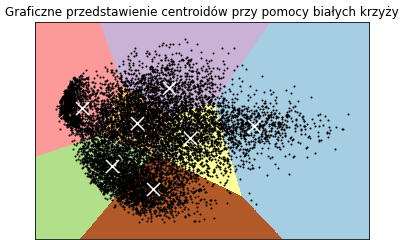
\includegraphics[scale=1.0]{k7}
	      \centering
	      \caption{Wszystkie wierzchołki ze zbioru treningowego}
	    \end{figure}
	    \begin{figure}[H]
	      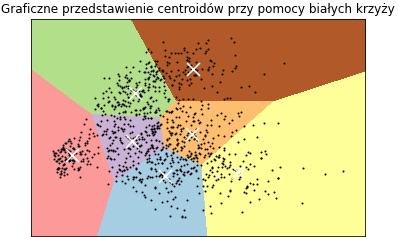
\includegraphics[scale=1.0]{k71000}
	      \centering
	      \caption{Wszystkie wierzchołki ze zbioru treningowego, ograniczenie: 1000 elementów}
	    \end{figure}
	    \item k=8 
		\begin{figure}[H]
	      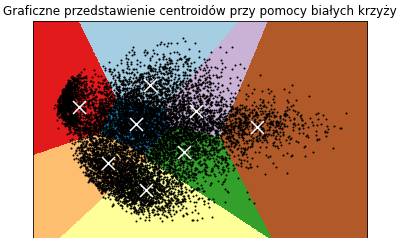
\includegraphics[scale=1.0]{k8}
	      \centering
	      \caption{Wszystkie wierzchołki ze zbioru treningowego}
	    \end{figure}
	    \begin{figure}[H]
	      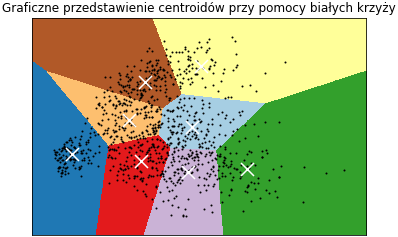
\includegraphics[scale=1.0]{k81000}
	      \centering
	      \caption{Wszystkie wierzchołki ze zbioru treningowego, ograniczenie: 1000 elementów}
	    \end{figure}
	    \item k=9 
		\begin{figure}[H]
	      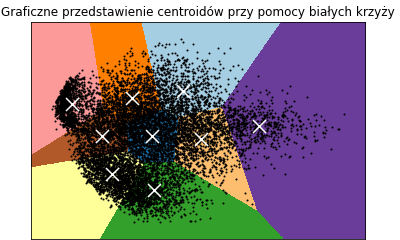
\includegraphics[scale=1.0]{k9}
	      \centering
	      \caption{Wszystkie wierzchołki ze zbioru treningowego}
	    \end{figure}
	    \begin{figure}[H]
	      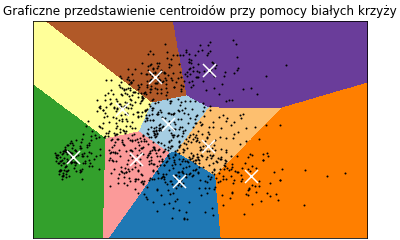
\includegraphics[scale=1.0]{k91000}
	      \centering
	      \caption{Wszystkie wierzchołki ze zbioru treningowego, ograniczenie: 1000 elementów}
	    \end{figure}
	    \item k=10 
		\begin{figure}[H]
	      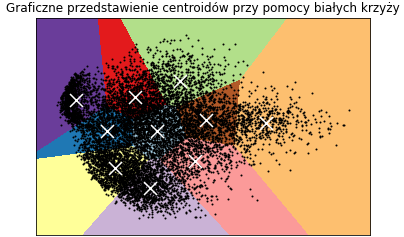
\includegraphics[scale=1.0]{k10}
	      \centering
	      \caption{Wszystkie wierzchołki ze zbioru treningowego}
	    \end{figure}
	    \begin{figure}[H]
	      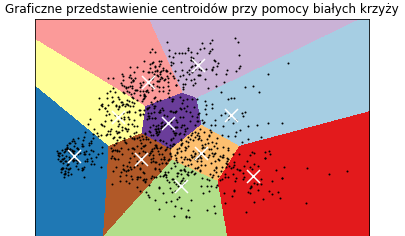
\includegraphics[scale=1.0]{k101000}
	      \centering
	      \caption{Wszystkie wierzchołki ze zbioru treningowego, ograniczenie: 1000 elementów}
	    \end{figure}
	    \item k=11 
		\begin{figure}[H]
	      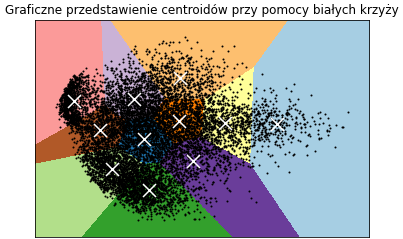
\includegraphics[scale=1.0]{k11}
	      \centering
	      \caption{Wszystkie wierzchołki ze zbioru treningowego, ograniczenie: 1000 elementów}
	    \end{figure}
	    \begin{figure}[H]
	      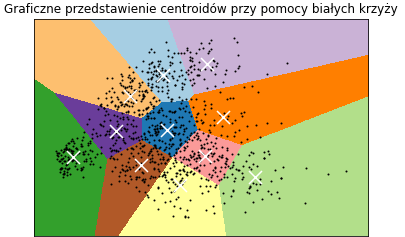
\includegraphics[scale=1.0]{k111000}
	      \centering
	      \caption{Wszystkie wierzchołki ze zbioru treningowego, ograniczenie: 1000 elementów}
	    \end{figure}
	    \item k=12
		\begin{figure}[H]
	      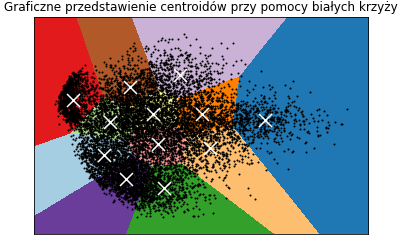
\includegraphics[scale=1.0]{k12}
	      \centering
	      \caption{Wszystkie wierzchołki ze zbioru treningowego, ograniczenie: 1000 elementów}
	    \end{figure}
	    \begin{figure}[H]
	      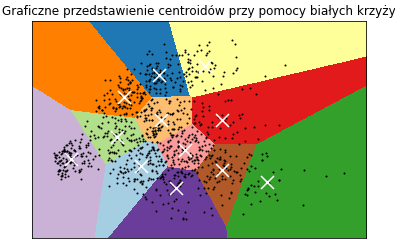
\includegraphics[scale=1.0]{k121000}
	      \centering
	      \caption{Wszystkie wierzchołki ze zbioru treningowego}
	    \end{figure}
	\end{itemize}
	\textbf{Obserwacja: } Widoczne punkty w obrębie klastrów nie układają się w cyfry
\section{Wykres inercji}
	\begin{figure}[H]
	      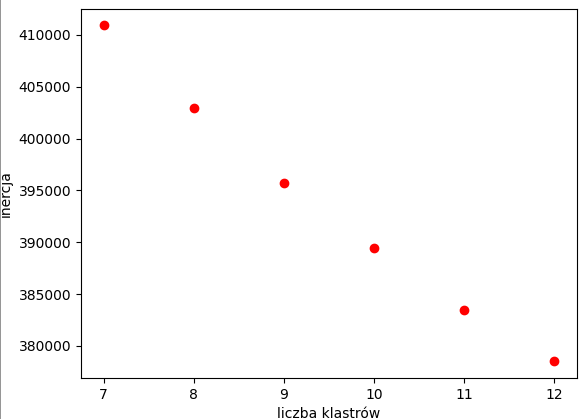
\includegraphics[scale=1.0]{klastry}
	      \centering
	      \caption{Wszystkie wierzchołki ze zbioru treningowego}
	    \end{figure}


\end{document}